
\chapter{EDA: review and extensions}

% contingency table margins
% notched boxplots
% heatmaps
% scatterplot matrices
% facets

\index{Exploratory Data Analysis (EDA)}
\index{univariate}
\index{bivariate}
\index{multivariate}

In this chapter, we'll review the \textbf{EDA} (\textbf{Exploratory Data
Analysis}) material you learned in DATA 101, and also present a few additional
techniques.

Remember, when you're first exploring some data, the first and most basic
questions to ask are:

\begin{compactenum}

\item Is the data \textbf{univariate} or \textbf{bivariate} (or
\textbf{multivariate})?\footnote{``Univariate'' data means that you're looking
at only one variable, even if there are many observations of that variable. A
bunch of people's SAT scores comprises a univariate data set, as does a bunch
of political affiliations, salaries, or declared majors. ``Bivariate'' data
contains \textit{two} pieces of information for \textit{each} observation: if I
have data about both the SAT score and the college GPA for each of a bunch of
students, that's a bivariate data set. Another example: a data set with both
the gender and the salary for each of a bunch of adults.}

\item Is it \textbf{categorical} or \textbf{numerical}?\footnote{Recall that a
``categorical'' variable is qualitative, typically chosen from a set of
possible values. Gender, political affiliation, and declared major are all
examples. ``Numerical'' variables are numbers (duh): salary, GPA, SAT score.
Numerical variables can further be refined by their scale of measure (ordinal,
interval, ratio), although that often doesn't affect the appropriate type of
exploratory statistics and plots too much.}

\end{compactenum}

The answers to these questions determines what kind of \textbf{statistic} is
relevant, and what kind of \textbf{plot} is appropriate.

\pagebreak
Example: let's say we're exploring a data set of great works of literature:

\begin{Verbatim}[fontsize=\small,samepage=true,frame=single,framesep=3mm]
books.iloc[0:5,:]
\end{Verbatim}
\vspace{-.2in}

\begin{Verbatim}[fontsize=\small,samepage=true,frame=leftline,framesep=5mm,framerule=1mm]
                       gender  year     lang   words
name                                                
Jane Eyre                   F  1847  English  183858
The Brothers Karamazov      M  1879  Russian  364153
Anna Karenina               M  1877  Russian  349736
The Inferno                 M  1320  Italian   45750
Huck Finn                   M  1884  English  109571
\end{Verbatim}

For each book, we have the \texttt{gender} of the author, the \texttt{year}
and \texttt{language} in which it was written, and the total number of
\texttt{words} it contains. Clearly \texttt{gender} and \texttt{lang} are
categorical variables, while \texttt{year} and \texttt{words} are numeric.

\section{Case 1: univariate categorical data}
\label{contingencyTable}
\index{contingencyTable}

\index{value\_counts@\texttt{.value\_counts()} (Pandas)}

When looking at just one variable, which is categorical in nature, the
appropriate analysis is the \textbf{one-dimensional contingency table}, which
shows the counts of the various values. Let's create a contingency table for
the book languages, using Pandas' \texttt{.value\_counts()} function:

\begin{Verbatim}[fontsize=\small,samepage=true,frame=single,framesep=3mm]
books['lang'].value_counts()
\end{Verbatim}
\vspace{-.2in}

\begin{Verbatim}[fontsize=\small,samepage=true,frame=leftline,framesep=5mm,framerule=1mm]
French     299
English    247
Spanish    217
Russian    150
Italian     92
Name: lang, dtype: int64
\end{Verbatim}

The most appropriate plot is a \textbf{bar chart} of these counts, which you
can create by simply tacking \texttt{.plot(kind="bar")} at the end:

\begin{Verbatim}[fontsize=\small,samepage=true,frame=single,framesep=3mm]
books['lang'].value_counts().plot(kind="bar")
\end{Verbatim}

\begin{center}
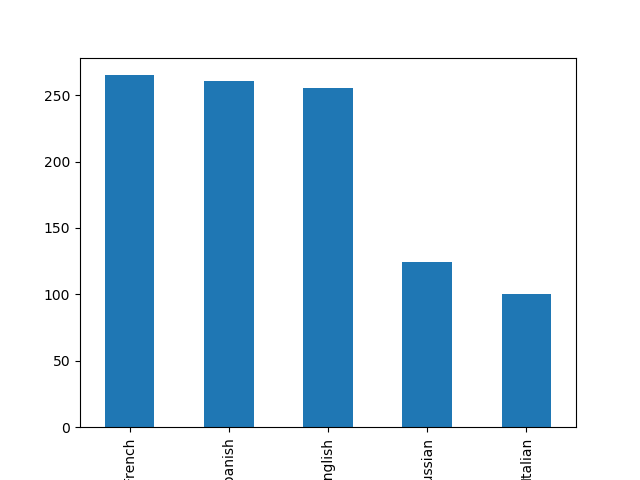
\includegraphics[width=0.6\textwidth]{barplot.png}
\end{center}

\section{Case 2: univariate numeric data}

\index{mean}
\index{standard deviation}
\index{quantiles}

When your single variable of interest is numeric, as is the \texttt{words}
column, the appropriate statistics are \textbf{mean}, \textbf{standard
deviation}, and the various \textbf{quantile} statistics (\textbf{minimum},
\textbf{.25 quantile},  \textbf{median}, \textbf{.75 quantile}, and
\textbf{maximum}):

\begin{Verbatim}[fontsize=\small,samepage=true,frame=single,framesep=3mm]
books['words'].mean()
books['words'].std()
books['words'].quantile([0,.25,.5,.75,1])
\end{Verbatim}
\vspace{-.2in}

\begin{Verbatim}[fontsize=\small,samepage=true,frame=leftline,framesep=5mm,framerule=1mm]
436739.737
232384.719
0.00      5443.0
0.25    241492.0
0.50    462552.0
0.75    637765.0
1.00    805341.0
\end{Verbatim}

Translation: on average, the books in our data set each have about 436,739
words, and if distributed normally (which we haven't checked yet) about
$\frac{2}{3}$rds of them are in the range 436,739 $\pm$ 232,384 (or between
204355 and 669123 words). The shortest book has 5443 words, the longest a
whopping 805,341, and half the books in the data set have 462,552 or less. A
quarter of the books have fewer than 241,492 words, and three quarters have
fewer than 637,765.

\index{histogram}

The best plot in this case is the \textbf{histogram}:

\begin{Verbatim}[fontsize=\small,samepage=true,frame=single,framesep=3mm]
books['words'].plot(kind="hist",bins=30)
\end{Verbatim}

which shows the entire ``lay of the land'' of the distribution of values.
Remember to experiment with the number of \texttt{\textbf{bins}}, since you
can get very different pictures of how the data is distributed depending on
your bin size (more on that in Lesson~\ref{ch:KDEs}).

\begin{center}
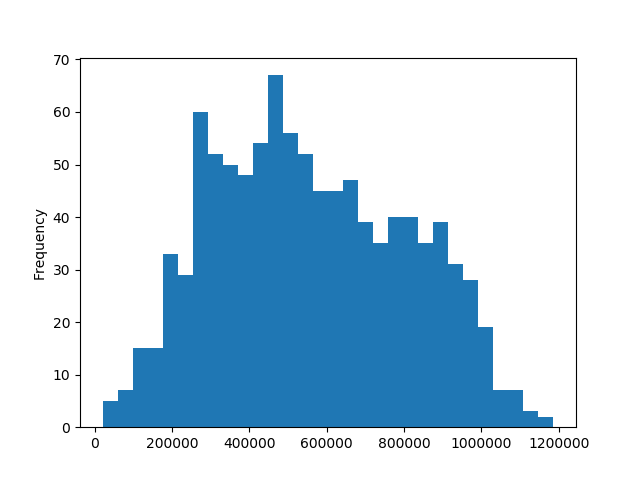
\includegraphics[width=.7\textwidth]{histogram.png}
\end{center}

\section{Case 3: bivariate data: categorical--categorical}

\index{groupby@\texttt{.groupby()} (Pandas)}

If you want to explore the relationship between two different variables, both
of which are categorical, you need a \textbf{two-dimensional contingency
table}. You can use \texttt{.value\_counts()} again in conjunction with
\texttt{.groupby()}):

\begin{Verbatim}[fontsize=\small,samepage=true,frame=single,framesep=3mm]
books.groupby('gender')['lang'].value_counts()
\end{Verbatim}
\vspace{-.2in}

\begin{Verbatim}[fontsize=\small,samepage=true,frame=leftline,framesep=5mm,framerule=1mm]
gender  lang   
F       French      79
        English     52
        Spanish     34
        Italian     29
        Russian     11
M       French     209
        English    196
        Spanish    193
        Russian    115
        Italian     87
Name: lang, dtype: int64
\end{Verbatim}

\index{crosstab@\texttt{.crosstab()} (Pandas)}

which shows, for each \texttt{gender}, how many books in each \texttt{lang} are
in the data set. I personally think the \texttt{pd.crosstab()} function is a
bit easier on the eyes for this, though:

\texttt{gender\_lang@\texttt{gender\_lang}}

\begin{Verbatim}[fontsize=\small,samepage=true,frame=single,framesep=3mm]
gender_lang = pd.crosstab(books['lang'], columns=books['gender'])
print(gender_lang)
\end{Verbatim}
\vspace{-.2in}

\begin{Verbatim}[fontsize=\small,samepage=true,frame=leftline,framesep=5mm,framerule=1mm]
gender    F    M
lang            
English  52  196
French   79  209
Italian  29   87
Russian  11  115
Spanish  34  193
\end{Verbatim}


\subsection{Margins: raw counts}
\label{marginsBegin}
\index{margins (of a contingency table)}
\index{raw counts@``raw'' counts}

\index{crosstab@\texttt{.crosstab()} (Pandas)}

The \texttt{pd.crosstab()} function is also useful for computing
\textbf{margins}, or row/column aggregate information. The easy part is to
include ``\texttt{margins=True}'' as an argument to \texttt{pd.crosstab()}. The
tricky part is understanding the different ways of presenting the margins,
since they're each subtly different and often confused. So heads up. Our first
use of margins will be to simply compute \textbf{raw counts}:

\begin{Verbatim}[fontsize=\footnotesize,samepage=true,frame=single,framesep=3mm]
gender_lang = pd.crosstab(books['lang'], columns=books['gender'], margins=True)
print(gender_lang)
\end{Verbatim}
\vspace{-.2in}

\begin{Verbatim}[fontsize=\small,samepage=true,frame=leftline,framesep=5mm,framerule=1mm]
gender     F    M   All
lang                   
English   52  196   248
French    79  209   288
Italian   29   87   116
Russian   11  115   126
Spanish   34  193   227
All      205  800  1005
\end{Verbatim}

In this table, the margins are \textit{total counts for each row, and for each
column.} Inspect the table and verify this is so: for each row (say,
\texttt{English}) the sum of the \texttt{F} entry (52) and \texttt{M} entry
(196) is equal to the total in the \texttt{All} entry (248). Similarly, the sum
of the entire first column (the \texttt{F}'s for all languages, which are 52,
79, 29, 11, and 34) is equal to the \texttt{All} element of that column (205).
And of course, the sum of the \texttt{All} rows -- or \texttt{All} columns,
same diff -- is the grand total of 1005.

\subsection{Margins: overall percentages}

Now suppose we \textit{divide every value of this table} by the grand total.
(We could literally divide by the number 1005, or divide by
\texttt{gender\_lang.loc[\textquotesingle All\textquotesingle
][\textquotesingle All\textquotesingle ]}, since that's how to programmatically
obtain the value of the bottom-right-hand entry.) This gives us \textbf{overall
proportions}, and if we multiply by 100, \textbf{overall percentages}:

\begin{Verbatim}[fontsize=\small,samepage=true,frame=single,framesep=3mm]
print(gender_lang / gender_lang.loc['All']['All'] * 100)
\end{Verbatim}
\vspace{-.2in}

\begin{Verbatim}[fontsize=\small,samepage=true,frame=leftline,framesep=5mm,framerule=1mm]
gender       F      M     All
lang                         
English   5.17  19.50   24.68
French    7.86  20.80   28.66
Italian   2.89   8.66   11.54
Russian   1.09  11.44   12.54
Spanish   3.38  19.20   22.59
All      20.40  79.60  100.00
\end{Verbatim}

Note carefully how to interpret this result: the sum total of all the table's
entries (except for those in the \texttt{All} row/column) is equal to 100\%.
This tells us that over $\frac{1}{5}$th (20.8\%) of all these books
\textit{were written in French by males}, only about 1\% of the books
\textit{were written in Russian by females}, and so forth.

\subsection{Margins: percentages by column}

By contrast, sometimes it's more helpful to have \textit{each column} add up to
100\%, rather than the entire table adding up to 100\%. You can accomplish this
like so:

\index{div@\texttt{.div() (NumPy)}}

\begin{Verbatim}[fontsize=\small,samepage=true,frame=single,framesep=3mm]
print(gender_lang.div(gender_lang.loc['All'],axis=1) * 100)
\end{Verbatim}
\vspace{-.2in}

\begin{Verbatim}[fontsize=\small,samepage=true,frame=leftline,framesep=5mm,framerule=1mm]
gender        F       M     All
lang                           
English   25.37   24.50   24.68
French    38.54   26.12   28.66
Italian   14.15   10.88   11.54
Russian    5.37   14.37   12.54
Spanish   16.59   24.12   22.59
All      100.00  100.00  100.00
\end{Verbatim}

(For now, the ``\texttt{.div()}'' call, and the ``\texttt{axis=1}'' thing, are
best to just follow verbatim rather than trying to understand what they mean.)

Notice that every \texttt{All} entry at the bottom is now equal to 100.
(The \texttt{All} entries on the right side are \textit{not}.) This view of
things allows us to see the language data \textit{on a per-gender basis}. For
instance, over 38\% \textit{of all the female authors} wrote in French, whereas
only 26\% \textit{of all the males} were in French.

\subsection{Margins: percentages by row}

We can do the corresponding process on a by-row basis by changing our syntax to
this:

\index{div@\texttt{.div() (NumPy)}}

\begin{Verbatim}[fontsize=\small,samepage=true,frame=single,framesep=3mm]
print(gender_lang.div(gender_lang['All'],axis=0) * 100)
\end{Verbatim}
\vspace{-.2in}

\begin{Verbatim}[fontsize=\small,samepage=true,frame=leftline,framesep=5mm,framerule=1mm]
gender       F      M    All
lang                        
English  20.97  79.03  100.0
French   27.43  72.57  100.0
Italian  25.00  75.00  100.0
Russian   8.73  91.27  100.0
Spanish  14.98  85.02  100.0
All      20.40  79.60  100.0
\end{Verbatim}

\underline{Important}: there are \textit{two} changes here from the previous
example, only one of which jumps out at you. The obvious one is that we have
``\texttt{axis=0}'' instead of ``\texttt{axis=1}''. But the one that's easy to
miss is that instead of ``\texttt{gender\_lang.loc[\textquotesingle
All\textquotesingle ]}'' we now have ``\texttt{gender\_lang[\textquotesingle
All\textquotesingle ]}'' (with \textit{no} ``\texttt{.loc}''). If you forget
this part, you'll get nonsense.

If you do it correctly, each \textit{row} (not column) will now sum to 100\%,
which gives us gender data \textit{on a per-language basis}. For example,
we can see that 91.27\% \textit{of the Russian books} were written by
men, but only 75\% \textit{of the Italian ones} were.

\subsection{\textit{Warning!}}

\index{statistical significance}
\index{$\chi ^2$ test}

Now you can stare at these numbers to get a feel for the them, and this is
encouraged. Remember, though, the proper way to test whether there's a
\textbf{statistically significant} relationship between two categorical
variables is to use a $\chi ^2$ test. And that leads me to mention a very
common pitfall.

\index{chi2\_contingency()@\texttt{chi2\_contingency()} (SciPy)}

Recall that when you call \texttt{scipy.stats.chi2\_contingency()}, you pass it
the contingency table. All well and good. But you must remember to pass it
\textit{the original contingency table \textbf{without} margins!} Once you've
started to compute and display margins, it's all too easy to forget that adding
margins \textit{adds a row and a column to the table} (for the ``\texttt{All}''
information) and if you give \texttt{chi2\_contingency()} this extraneous data
it messes up the whole $\chi ^2$ computation.

This is why in all the examples above, I deliberately did \textit{not} store
the ``margined'' version of the table back into the \texttt{gender\_lang}
variable. Instead, I kept only the table of raw counts in the variable, and
simply \textit{printed} the margined version when necessary, a la:

\begin{Verbatim}[fontsize=\small,samepage=true,frame=single,framesep=3mm]
# Correct!
gender_lang = pd.crosstab(books['lang'], columns=books['gender'])
print(gender_lang.div(gender_lang.loc['All'],axis=1) * 100)
scipy.stats.chi2_contingency(gender_lang)
\end{Verbatim}

I've seen plenty of well-intentioned students do this instead:

\begin{Verbatim}[fontsize=\small,samepage=true,frame=single,framesep=3mm]
# WRONG!
gender_lang = pd.crosstab(books['lang'], columns=books['gender']).div(
    gender_lang.loc['All'],axis=1) * 100)
print(gender_lang)
scipy.stats.chi2_contingency(gender_lang)
\end{Verbatim}

which leads to madness.

\subsection{(Not) plotting multiple categorical variables}

\index{mosaic plot}

Finally, what about plots for multiple categorical variables? Unfortunately,
the only plot I really know of for this is called a \textbf{mosaic plot}, and I
think they're so difficult to interpret that I don't really recommend them. Let
me know if you find a good alternative.

\label{marginsEnd}


\section{Case 4: bivariate data: categorical--numerical}

Suppose the two variables you're interested in are one categorical and one
numerical. For instance, maybe you're wondering whether men or women have
contributed more recent literary works, or which languages tend to have longer
longer books. 

\index{box plot}

The right plot here is the \textbf{box plot}, since it allows you to easily
compare groups. For the language vs.~length example:

\begin{Verbatim}[fontsize=\small,samepage=true,frame=single,framesep=3mm]
books.boxplot(column='words', by='lang')
\end{Verbatim}

\begin{center}
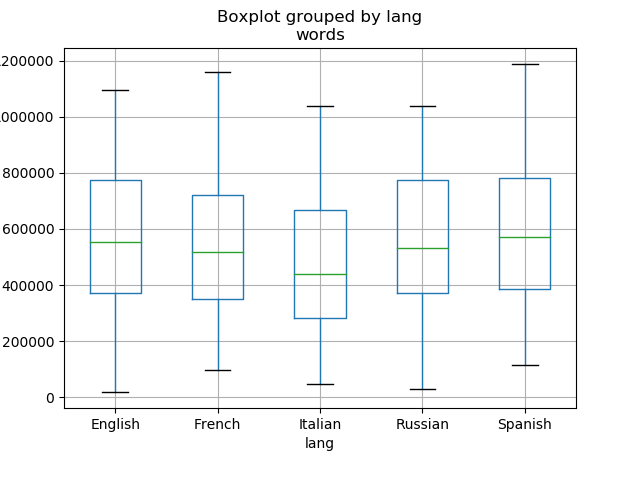
\includegraphics[width=0.8\textwidth]{boxplot.png}
\end{center}

\index{$t$-test}
\index{ttest\_ind@\texttt{ttest\_ind()} (SciPy)}

Apparently Italian works are a bit shorter than the other languages (especially
French), but it's hard to tell whether there's any truly significant difference
between the averages among the various groups. Recall that one way to find this
out is a \textbf{$t$-test for the difference of means}, using
\texttt{scipy.stats.ttest\_ind()}.

\index{box plot!notched}
\index{notched box plot}

Here's another way. You can use a \textbf{\textit{notched} boxplot}:
\label{notched}

\begin{Verbatim}[fontsize=\small,samepage=true,frame=single,framesep=3mm]
books.boxplot(column='words', by='lang', notch=True)
\end{Verbatim}

\index{statistical significance}

As long as your group sizes are big enough, this visually indicates whether or
not there is a stat sig diff between groups, based on \textit{whether the
notched areas overlap}. In the above case, the French and Italian notches
overlap, which means we can conclude \textit{nothing} reliable about French
works being longer than Italian ones. However, the Russian and Italian notches
do \textit{not} have any overlap, which means we \textit{should} feel confident
about declaring that on average, Russian works are longer than Italian ones.

\begin{center}
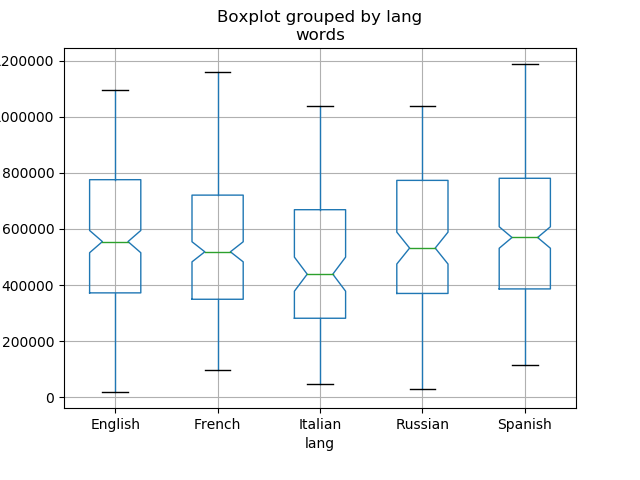
\includegraphics[width=0.9\textwidth]{notchedboxplot.png}
\end{center}

\section{Case 5: bivariate data: numerical--numerical}

\index{scatter plot}

Finally, the case where our two variables of interest are both numerical. The
obvious plot type here is the \textbf{scatter plot}, which shows one point for
each observation, with its $x$ and $y$ position determined by its values for
each variable.

\begin{Verbatim}[fontsize=\small,samepage=true,frame=single,framesep=3mm]
books.plot.scatter(x='year', y='words')
\end{Verbatim}

\index{Pearson correlation coefficient}
\index{correlation coefficient}

Clearly a big takeaway from the scatter plot below is that literary works have
been getting steadily shorter over the years. You'll remember that the
statistical reliability of this conclusion could be confirmed (or denied) by
taking a look at the Pearson's correlation coefficient.

\begin{center}
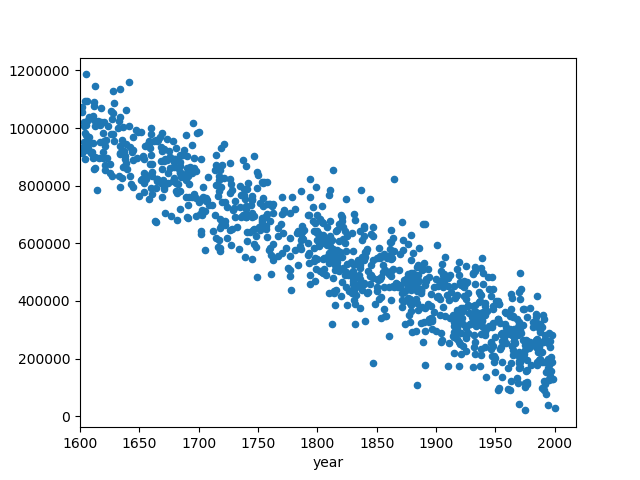
\includegraphics[width=0.9\textwidth]{scatterplot.png}
\end{center}

